\RequirePackage{luatex85}
\documentclass[tikz]{standalone}
% Default preamble
\usepackage{pgfplots}
\pgfplotsset{compat=newest}
\usepgfplotslibrary{groupplots}
\usepgfplotslibrary{polar}
\usepgfplotslibrary{smithchart}
\usepgfplotslibrary{statistics}
\usepgfplotslibrary{dateplot}
\usepgfplotslibrary{ternary}
\usepackage[T1]{fontenc}
\usepackage{lmodern}
\begin{document}
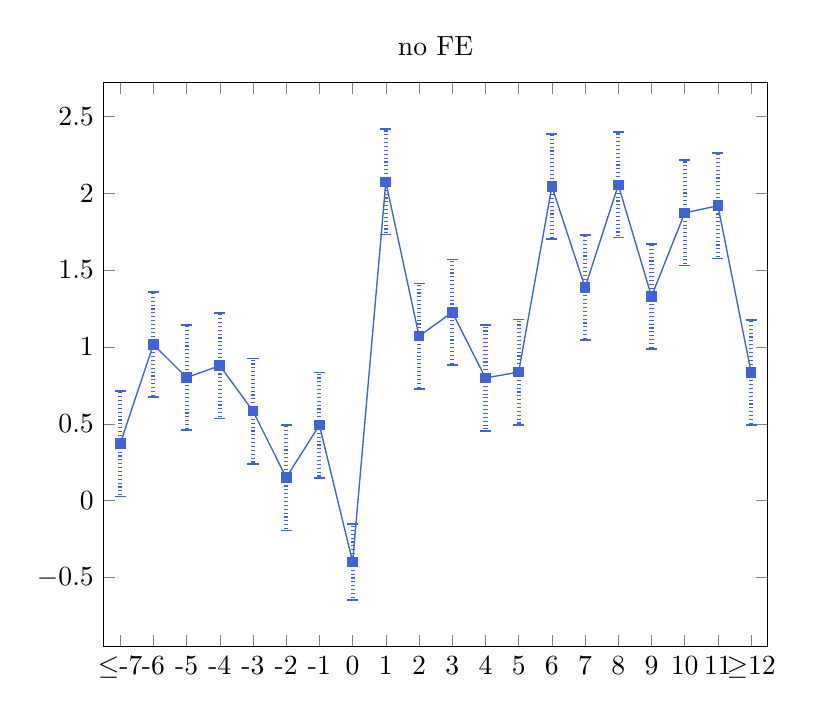
\begin{tikzpicture}
\begin{axis}[title={no FE}, title style={}, xlabel style={}, ylabel style={}, xticklabel style={}, yticklabel style={}, width={240pt}, height={204pt}, symbolic x coords={$\leq$-7,-6,-5,-4,-3,-2,-1,0,1,2,3,4,5,6,7,8,9,10,11,$\geq$12}, xtick={$\leq$-7,-6,-5,-4,-3,-2,-1,0,1,2,3,4,5,6,7,8,9,10,11,$\geq$12}, xmin={{[normalized]-0.5}}, xmax={{[normalized]19.5}}, scale only axis]
    \addplot[mark={square*}, mark options={mark size={1.75pt}, line width={0pt}, fill={rgb,255: red, 64; green, 99; blue, 216}, fill opacity={1}, draw={rgb,255: red, 64; green, 99; blue, 216}, draw opacity={1}}, error bars/error mark={|}, error bars/error mark options={mark size={2.0pt}, solid, line width={0.6pt}, fill={rgb,255: red, 64; green, 99; blue, 216}, fill opacity={1}, draw={rgb,255: red, 64; green, 99; blue, 216}, draw opacity={1}}, error bars/error bar style={draw={rgb,255: red, 64; green, 99; blue, 216}, draw opacity={1}, densely dotted, line width={1.5pt}}, draw={rgb,255: red, 64; green, 99; blue, 216}, draw opacity={1}, line width={0.5pt}, error bars/y dir={both}, error bars/y explicit]
        coordinates {
            ($\leq$-7,0.36968848040224767) +- (0,0.34267)
            (-6,1.0161642543359581) +- (0,0.34267)
            (-5,0.8004351374649978) +- (0,0.34267)
            (-4,0.8778993522840808) +- (0,0.34267)
            (-3,0.5827695112478881) +- (0,0.34267)
            (-2,0.14944225350724832) +- (0,0.34267)
            (-1,0.49160731110003014) +- (0,0.34267)
            (0,-0.39846952781011685) +- (0,0.24537)
            (1,2.0726463666986965) +- (0,0.34267)
            (2,1.069919698272852) +- (0,0.34267)
            (3,1.2250710642968259) +- (0,0.34267)
            (4,0.797671985702108) +- (0,0.34267)
            (5,0.8364708751691308) +- (0,0.34267)
            (6,2.0437448807973797) +- (0,0.34267)
            (7,1.385907470897294) +- (0,0.34267)
            (8,2.052924230676942) +- (0,0.34267)
            (9,1.3283311252365637) +- (0,0.34267)
            (10,1.8713616815794547) +- (0,0.34267)
            (11,1.917987763924949) +- (0,0.34267)
            ($\geq$12,0.8338398361407332) +- (0,0.34267)
        }
        ;
\end{axis}
\end{tikzpicture}
\end{document}
